\section{Evaluation}
\label{sec:evaluation}

In this section, we first present qualitative arguments to estimate storage requirements and traffic overhead, followed by results from a large-scale event-based simulation to study the query latency and load distribution in our scheme. We show that consistent hashing proportionally distributes the GUID:NA mapping such that the storage at any particular AS does not exceed feasible limits. We also find that the 95th percentile query latency is bounded below 100 ms using modest amount of replication, thus meeting the goal of fast resolution.

To analyze the storage requirements in absence of specifications about the GUID/NA lengths and related headers, we make the following assumptions. We assume flat GUIDs of length 160 bit, each associated with a maximum of 5 NAs (accounting for multi-homes devices) of length 32 bits each. 32 bits of additional overhead per mapping entry is assumed which could include type of service, priority and other side information. Each mapping entry thus has a size of 160 + 32x5 + 32 = 352 bits. We assume a total of 5 Billion GUIDs, roughly equal to the present number of mobile devices, and a replication factor of $K = 5$. Based on the average prefix announcement by individual ASs as determined from a current snapshot of the BGP table~\cite{dix-ie}, the storage requirements per AS, assuming roughly proportional distribution, is only 173 Mbits.

The update traffic overhead is also a key parameter of interest in ensuring scalability. The DIHT technique reduces the traffic overhead in comparison to other mapping schemes by: (a) Ensuring single overlay-hop path to storage location, (b) Not adding any table maintenance traffic as required in DHT based schemes. Using a broad estimate of 50\% of the 5 Billion GUIDs being those of mobile hosts which update their GUID:NA mapping at an average rate of 100 updates/day, the world-wide combined update traffic would be $\sim$5 Gb/s, a minute fraction of the overall Internet traffic of $\sim 50$x$10^6$ Gb/s as of 2010~\cite{cisco}.

Next we describe our event-based simulation setup and present results which characterize the critical parameters of query latency and load distribution for our scheme.

\subsection{Simulation setup}
\label{subsec:evaluation_setup}

\subsubsection{Event-based Simulator Architecture}
%\begin{figure}[h]
%\centering
%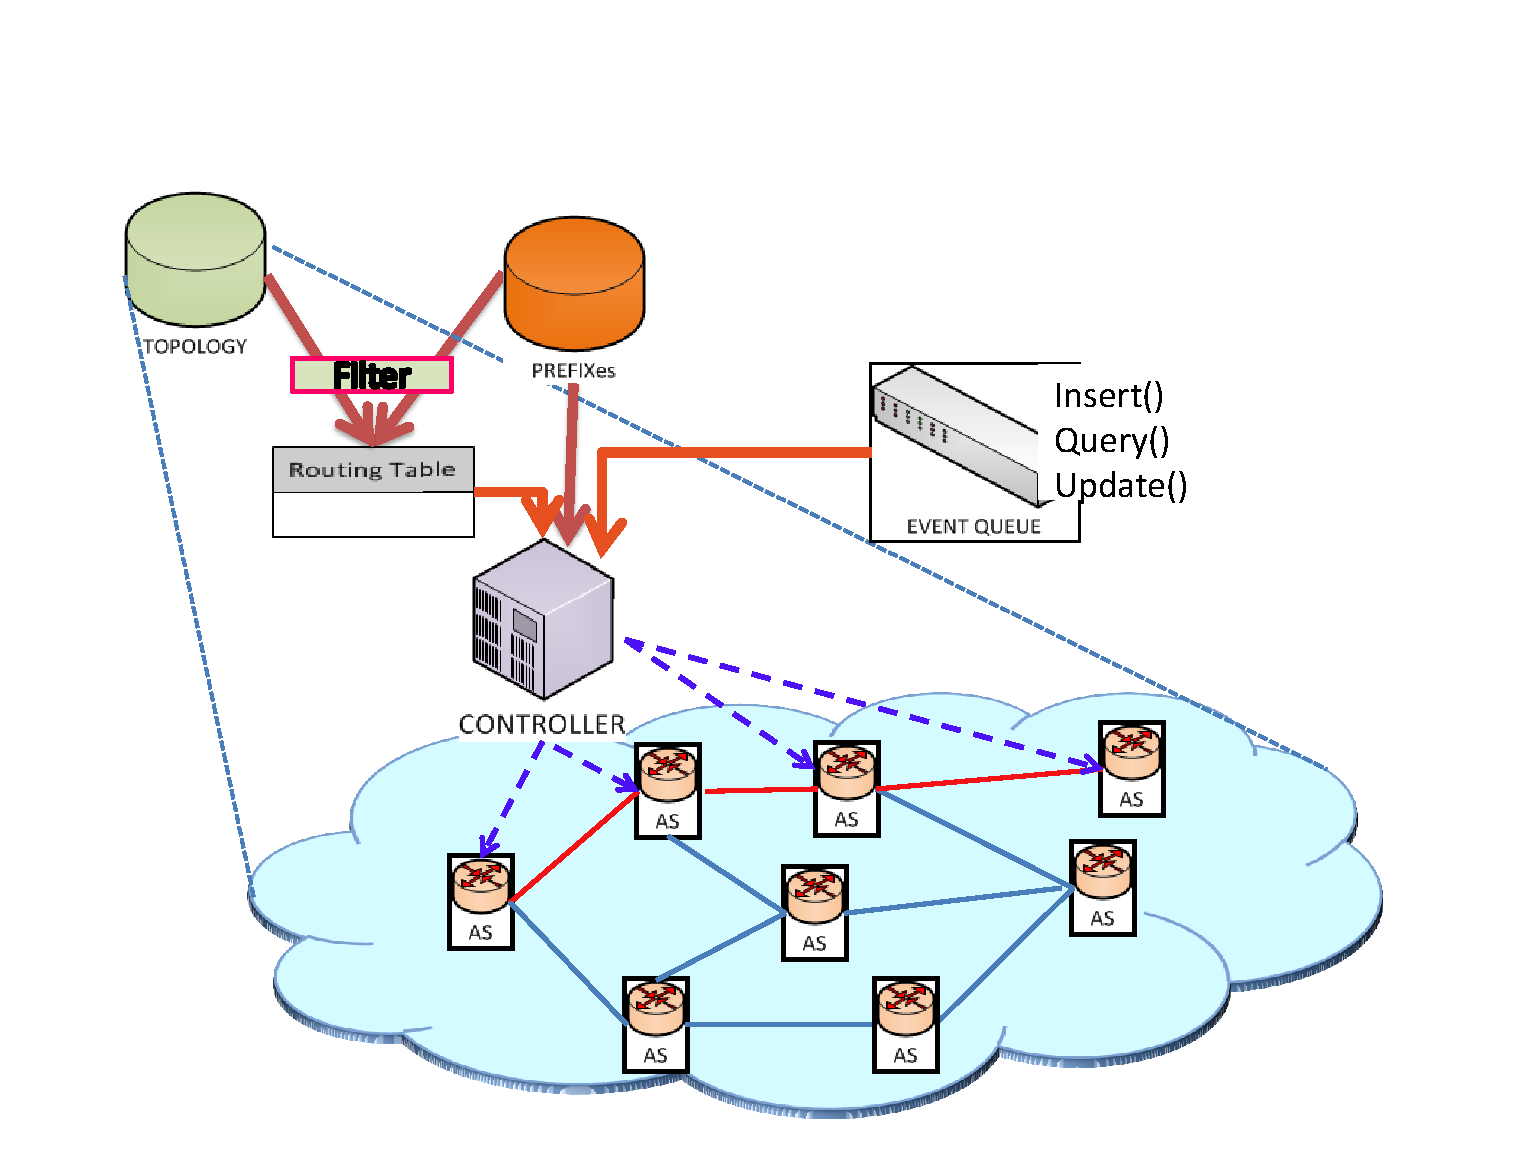
\includegraphics[width=0.5\textwidth]{figures/Simmulation_setup.eps}
%\caption{Simulation Setup}
%\label{fig:simulator}
%\end{figure}

The discrete-event simulator consists of $\sim$26000 nodes, each of which emulates the relevant operations of an individual AS. The connectivity graph of the network, inter-AS and intra-AS connectivity latencies, and the announced IP prefix list are derived from measurement driven data as described in Section~\ref{subsubsec:dataSources}. Three types of event:  GUID inserts, GUID updates and GUID lookups are pre-generated and organized into a global queue.  The global queue guarantees that the order of events on each run are the same and will lead to the same outcome. The event controller processes events in the global queue in sequential order following the sequence of operations outlined in~\ref{sec:design} to process each kind of event. For each query event, the total latency is computed and stored as a data point. The simulation concludes with data gathering from each AS in terms of number of GUIDs stored and average query/update rates.
\footnote{The source code for our simulation is made available at \cite{sourceCode_NRS}}

%It then produces a inter-domain routing table for all ASes in the network. We consider that each AS has one participating BGP router.

\subsubsection{Data Sources}
\label{subsubsec:dataSources}
We use the AS-level topology of the current Internet as our network model by extracting the following real-measurement data from the DIMES database~\cite{shavitt}: (i) Connectivity graph containing 26,424 ASs and 90,267 direct links between them, (ii) Average end-to-end latencies between each pair of AS and within each AS. The DIMES database provides end-to-end median latency for about 9 million pairs of hosts which are either within the same AS or in different ASs. From this dataset, we extract the average inter-AS and intra-AS latency since we only work with a AS-level network topology in our simulation. Due to the inherent incompleteness of real-trace data, intra-AS latency numbers are not available for about 6\% of the ASs that are involved in the storage or transit of the mapping data. For these ASs, we use the median value (3.5 ms) of the set of available intra-AS latencies as a working solution. We note that there are other measurement driven sources for AS topology data, for example~\cite{madhyastha} and~\cite{claffy}, but we found DIMES to have a more complete view of the AS-level graph compared to any other database. For route selection, we use minimum latency paths between each pair of source and destination AS and make a conscious decision of not employing one of many path inference schemes such as~\cite{gao,weinsberg} that aim at also incorporating estimated policies at each AS. The dynamic nature of AS relationships, multi-homed networks and hidden/misconfigured policies prevalent in the Internet limits the accuracy of such schemes, introducing an uncharacterizable source of error in the results. We chose to present our results with the caveat of AS policy ignorance instead of adding unknown inference errors.

Since our scheme allocates GUIDs to ASs according to the prefix announcements, we use a complete list of IP prefixes advertised in the Internet default free zone, as seen by APNIC's router at DIX-IE in Tokyo, Japan~\cite{dix-ie}. This dataset consists of roughly 330,000 prefixes spanning close to 52\% of the 32 bit IP address space which is consistent with recent estimates~\cite{elmokashfi} about the size of the prefix tables in DFZ routers. We confirm our results with two other prefix tables taken from BGP routers in the continental USA and Europe respectively and observe similar trends.

To discard any location bias and to incorporate the global scale of operation, we use another dataset from DIMES to characterize the distribution of the source of GUID insert and query. Each GUID in our simulation is originated from a randomly picked source AS, where the probability of choosing a certain AS is weighted in proportion to the number of end-nodes found in that AS as per the DIMES database. The end-result emulates a real deployment scenario in which more populated areas (characterized by high number of IP end-nodes) will generate more GUID queries compared to less populated areas. We note that the nature of trace collection employed by DIMES might introduce a bias due to non-uniformity of vantage point distribution (though shown to be small), however we do not take this into account in our simulation.

\subsection{Results}
We present two sets of results that characterize the query latency and the load distribution of our scheme respectively.

\subsubsection{Query Latency}
The most critical performance measure of a mapping scheme is the delay incurred between making a query and receiving a reply from the appropriate mapping source. Low query latency is a key requirement for efficient mobility support using the name and locator split mechanism. We characterize the query latency of our scheme by running a set of simulations as per Section~\ref{subsec:evaluation_setup} with 100K GUID inserts and queries and varying values for the replication factor $K$, from 1 to 5. By repeated trials, we verified that the latency averages converge with 100K data points and further increasing the number of queries does not provide any additional insights. Figure~\ref{fig:queryLatency} plots the Cumulative Distribution Function (CDF) of the round trip query latency for different values of $K$. The effect of increasing $K$, as described in Section~\ref{subsubsec:replication} can be clearly seen with the leftward shift of the CDF curve as we increase the value of $K$. In particular, the mean, median and $95^{th}$ percentile query latencies of $K = 1$ and $K = 5$ cases are tabulated in Table~\ref{table:latency} which shows a marked decrease in the tail of the latency distribution. The low query latency values and a relatively thin tail distribution for $K = 5$ validates the effectiveness of our scheme and shows that it can be used even under very stringent latency requirements.
\begin{center}
\begin{figure}[h]
%\vspace{-0.2in}
\centering
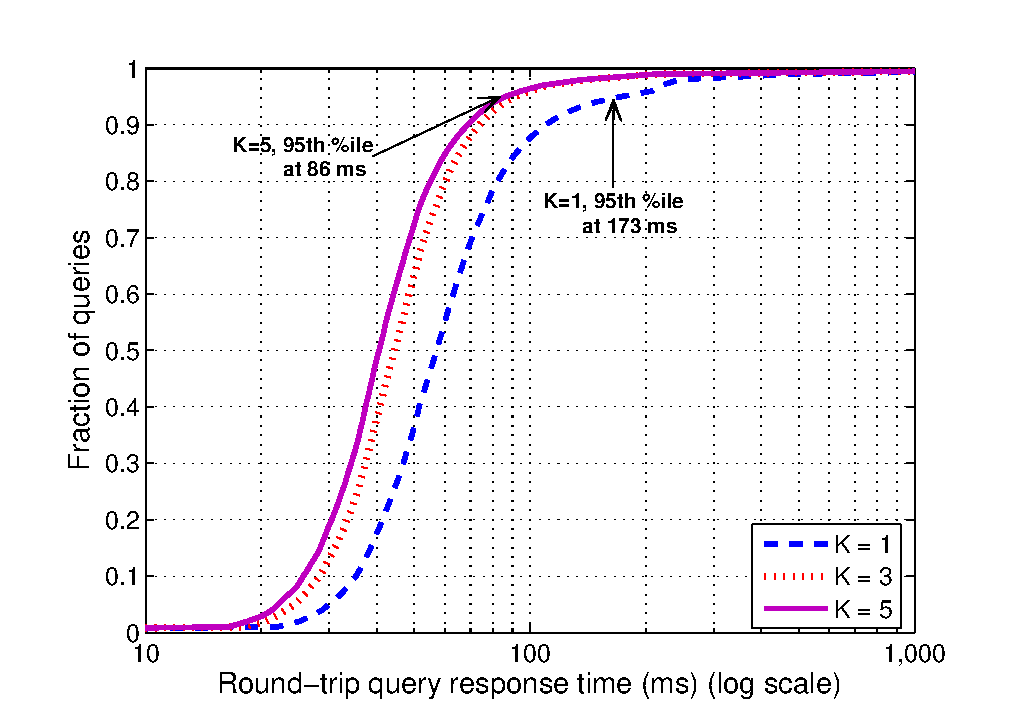
\includegraphics[width=0.5\textwidth]{figures/queryLatency}
\caption{Empirical CDF of the round trip query latency}
\label{fig:queryLatency}
%\vspace{-0.2in}
\end{figure}
\end{center}
%Possible optimizations leading to further reduction in the latency are discussed in Section [?]
\begin{table}[t]
%\vspace{-0.2in}
\centering
\begin{tabular}{|c|c|c|c|}
\hline
\multicolumn{1}{|c|}{$K$} & \multicolumn{3}{|c|}{Round Trip Query Latency(ms)}\\
\cline{2-4}
 & Mean & Median & 95th percentile\\
\hline
1 & 77.8 & 57.9 & 202.0\\
\hline
5 & 51.3 & 41.7 & 90.9\\
\hline
\end{tabular}
\caption{Query Latency Statistics for $K $ = 1, 5}
%\vspace{-0.2in}
\label{table:latency}
\end{table}

\subsubsection{Load Distribution}
To ensure that the scheme scales and no particular AS is assigned a disproportionally large number of GUIDs, fairness in load distribution is an important factor. Using the current IP addresses as an example of the NA space, we show that despite the heavily fragmented allocation of this space, our scheme exhibits fairness of GUID assignments. We measure fairness in terms of the Normalized Load Ratio (NLR) at each AS, which is defined as the ratio of GUID percentage assigned to that AS over the IP percentage advertised by that AS. For example if an AS announces a $/8$ prefix, corresponding to 0.39\% of the 32 bit IP space and gets assigned 20,000 out of a total of 1 Million GUIDs i.e 2\% of GUIDs, then its normalized load would be 2/0.39 $\simeq$5.

To evaluate the load distribution, we run a second experiment with 10 Million GUID inserts and a fixed value of $K = 1$. A higher number of inserts provide sufficient number of data points for averaging which is required to cover the wide variability in the number and size of IP prefix announcements. Simulations with higher values of $K$ show similar trends and we only present the $K = 1$ case for clarity.
Figure~\ref{fig:loadDistr} shows the CDF of the normalized load over all the ASs in the network for this simulation. Close to 70\% of the ASs lie in the flat vertical portion of the curve, indicating a fair assignment with narrow tails. The median NLR value of $\sim$2 is expected since in addition to its fair share of GUIDs, each AS is also allocated a portion of the GUIDs that fall in the IP holes as described in Section~\ref{subsec:ip_hole}. We note that as we further increase the number of inserts, the tail distributions become narrower and the distribution of NLR values asymptotically converges to a fixed value.

\begin{center}
\begin{figure}[h]
%\vspace{-0.2in}
\centering
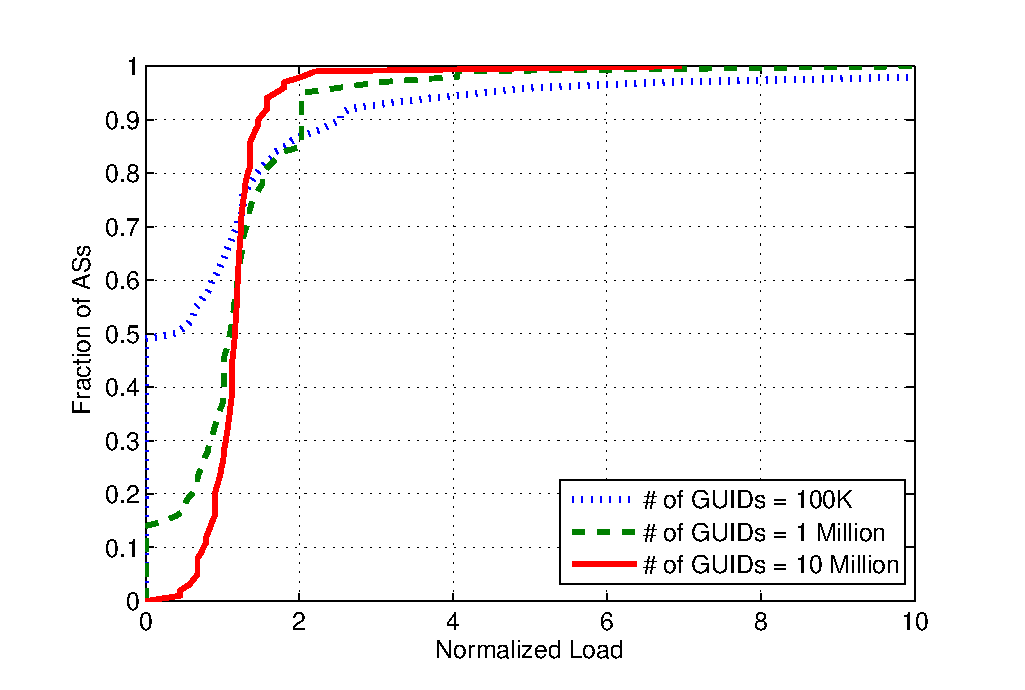
\includegraphics[width=0.5\textwidth]{figures/loadDistr}
\caption{Empirical CDF of normalized Load per AS}
\label{fig:loadDistr}
\vspace{-0.2in}
\end{figure}
\end{center}

%This section present our large scale simulation implementation.

%Our simulation takes description of the network topology at layer-3 from netDimes \cite{} including 90 thousands single-hop AS-to-AS connection, from which we build the connectivity graph between ASes. We derives from 9 Millions  end-to-end traces from netDimes to have an estimation of intra-AS latency for every AS. Let $L_{AS1}$ and $L_{AS2}$ are intra AS latency of AS1 and AS2 accordingly.  If there is a connectivity from AS1 to AS2, the latency for every single-hop AS-to-AS connection is compute as follow.

%We takes a list of IP prefixes from \cite{}, a Japanese BGP border gateway. it produces a inter-domain routing table for all routers in the network. That route selection process computes the shortest path according to  from the provided topology. One might argues that the route selection should follow BGP which also takes ASes' policies into account. However,  for simplicity, all policies should be reflected on the provided topology in our model, e.g. if an AS prefers one path over another, that preference should be represented in path's cost. Note that edges are directional.

%Once the topology is loaded, and the inter-domain routes have been computed, the Actuator starts processing events in global queue in sequential order. The global queue guarantees that the orders of events on each run are the same and will lead to the same outcome. That is in contrast with traditional discrete event where outcome depends on the seed of the pseudo random number generator. There are several types of events, including  GUID insert, GUID update, GUID lookup and BGP table update.

%For each insertion event extracted from the global even queue, Actuator applies k hash function on to that GUID, may rehash up to m times to get the hashed value felt into announced IP address, called IPx. For each IPx, Actuator lookup on AS prefix table to find the corresponding AS and destination IP address of BGP speaker's of that AS. It then get the list of  ASes that the request must be directed through in order to be delivered to that destination AS. For each AS on the path, Actuator updates the message counter of that AS, adjust the time stamp on that AS, and increase the time stamp for that request based on the latency of the passed through link. For timestamp adjustment on particular AS, Actuator assign the greater timestamp among <AS time stamp, message time stamp>  as the new time stamp for that AS. The message is forwarded on a AS-by-AS basis until it reaches its final destination. Upon delivered to the destination, destination AS update its GUID list with the new one, followed by GUID's time stamp.

%The actuator continues the simulation by popping the first event from the global queue, simulating the behavior at each router along the path. If the event is GIUD lookup or GIUP date, the steps tobe executed by the actuator are very much similar to that with aforementioned GUID insert.  If the event is BGP table update, the actuator takes the diff operation to compare the old table with the new one. It then identifies ASes that got affected from the change�
